\documentclass[ITR,BA,english,intermediate,tutorial]{LSR_thesis} 
\graphicspath{{pics/}}

%% Options:
%% LSR: LSR Template with Prof. Buss as default
%% ITR: ITR Template with Prof. Hirche as default

%% BA: Bachelorarbeit / Bachelor thesis
%% MA: Masterarbeit / Master thesis
%% HS: Hauptseminar / Scientific seminar
%% PP: Projektpraktikum / practical course
%% IP: Ingenieurpraxis
%% FP: Forschungspraxis
%% SeA: Semesterarbeit (MW)

%% english
%% german

%% final
%% intermediate

%% tutorial -> remove flag such that help files and todos are removed

%%% last changes: 7.02.2019 (v.gabler@tum.de)

%------------------------------------------------%
%_________CUSTOMIZE LATEX ONLY IN customize.tex!_% 
%_________ DO NOT MODIFY THE TEMPLATE!___________%
%________________________________________________%
% add customize first so you can access your commands in gloss, or fuse both into one file
%%%%%%%%%%%%%%%%%%%%%%%%%%%%%%%%%%%%%%%%%%%%%%%%%%%%%%%%%%%%%%
% CUSTOMIZING Tex-File for students to be adjusted as needed %
%%%%%%%%%%%%%%%%%%%%%%%%%%%%%%%%%%%%%%%%%%%%%%%%%%%%%%%%%%%%%%
%%%%%%%%%%%%%%%%%%%%%
% CUSTOM PACKAGES	%
%%%%%%%%%%%%%%%%%%%%%
\usepackage{tikz}
\usepackage{pgfplots}

%%%%%%%%%%%%%%%%%%%%%
% CUSTOM COMMANDS	%
%%%%%%%%%%%%%%%%%%%%%
% e.g. Math conventions as vectors, Matrices, sets
\renewcommand{\vec}[1]{\mathbf{\MakeLowercase{#1}}}
\newcommand{\Mat}[1]{\mathbf{\MakeUppercase{#1}}}
\newcommand{\set}[1]{\boldsymbol{#1}}

% e.g. use differenc layers in tikz
\pgfdeclarelayer{background}
\pgfdeclarelayer{nodelayer}
\pgfdeclarelayer{edgelayer}
\pgfdeclarelayer{foreground}
\pgfsetlayers{background,edgelayer,nodelayer,main,foreground}
%%%%%%%%%%%%%%%%%%%%%
% HYPHENATIONS 		%
%%%%%%%%%%%%%%%%%%%%%
\hyphenation{Lya-pu-nov}

 % add custom commands etc in this file 
% %%%%%%%%%%%%%%%%%%%%%%%%%%%%%%%%%%%%%%%%%%%%%%%%%%%%%%%%%%%%%%
% NOTE: Using this is optional
% 	Nonetheless, feel free to include this file and adjust the 
% 	examples below as needed
%   
% Questions, feedback and improvements:
%	-> https://git.lsr.ei.tum.de/students/student-templates/issues
% ATTENTION:
% 	- Keep in mind that thif file uses the \vec and \mat commands
% 	 	which are defined in customize.tex!
%	- add glsaddall if you want all of the elements in gloss.aux
%		being printed into your list of acronyms.
% Further reading:
%	https://ctan.org/pkg/glossaries?lang=en
%%%%%%%%%%%%%%%%%%%%%%%%%%%%%%%%%%%%%%%%%%%%%%%%%%%%%%%%%%%%%%

% include packages
\usepackage{setspace}
\usepackage{filecontents}
% for sharelatex, the indexing using xindy:
% 	http://xindy.sourceforge.net/doc/faq-1.html#ss1.2
% is not available, thus the adjustments below ar necessary
%% Adjust Flag for Sharelatex
\newif\ifShareLatex 
%\ShareLatextrue            	% if you work in sharelatex: https://sharelatex.tum.de
\ShareLatexfalse          		% if you work locally

\ifShareLatex
    \usepackage[acronym, style=alttree, shortcuts, toc=true, nomain, nonumberlist]{glossaries}
    \renewcommand{\makeglossaries}{\makenoidxglossaries}
    \renewcommand{\printglossary}{\printnoidxglossary}
\else
    \usepackage[acronym,style=alttree, toc=true, shortcuts, xindy, nomain, nonumberlist]{glossaries}
    \RequirePackage[xindy]{imakeidx}
\fi

%%%%%%%%%%%%%%%%%%%%%%%%%%%%%%%%%%
% DEFINE HEADINGS AND CATEGORIES %
%%%%%%%%%%%%%%%%%%%%%%%%%%%%%%%%%%
% preferable use a command, to adjust the Capitalization 
% for the header section of fancyhdr automatically
\newcommand{\Symbols}{List of Symbols}
\newcommand{\Notation}{Notation}
\newglossary{symbols}{sym}{sbl}{\Symbols}
\newglossary{notation}{not}{nt}{\Notation}
% set width of first row
\glssetwidest{THISWIDE}     % adjust length as needed

%%%%%%%%%%%%%%%%%%%%%%%%%%%%%
% DEFINE ACRONYMS/GLOSSARY	%
%%%%%%%%%%%%%%%%%%%%%%%%%%%%%
\makeglossaries % don't remove this
\begin{filecontents}{gloss.aux}
	%===========%
	% ACRONYMS	%
	%===========%
	\newacronym{MPC}{MPC}{model-predictive control}
	\newacronym{BIBO}{BIBO}{bounded-input bounded-output}
	\newacronym{HRC}{HRC}{Human-Robot Collaboration}
	%============%
	% SYMBOLS	%
	%===========%
	\newglossaryentry{control}{type=symbols,
		sort={control},
		name={\ensuremath{\vec{u}}},
		description={control input vector}
	}
	%============%
	% NOTATION	%
	%===========%
	\newglossaryentry{vector}{type=notation,
		sort={vector},
		name={\ensuremath{\vec{x}_n}},
		description={$n$-dimensional vector named $x$}
	}	
	\newglossaryentry{matrix}{type=notation,
		sort={vector-matrix},
		name={\ensuremath{\Mat{x}_{m\times n}}},
		plural={matrices},
		user1={Mat},
		description={\ensuremath{m\times n} dimensional Matrix  named \ensuremath{X}}
	}	
\end{filecontents}
\loadglsentries{gloss.aux}

%%%% Add GLOSSARIES at end of thesis
\newcommand{\AddMyGloss}{
	\ifLSRITRtutorial
		\glsaddall 
	\fi
	\renewcommand{\glsglossarymark}[1]{}
   	\printglossary[type=acronym]
	\markboth{\MakeUppercase{acronyms}}{\MakeUppercase{acronyms}}
  	\ifdefined\Symbols
		\printglossary[type=symbols, nogroupskip]
		\markboth{\MakeUppercase{\Symbols}}{\MakeUppercase{\Symbols}}
	\fi
	\ifdefined\Notation
		\printglossary[type=notation, nogroupskip]
		\markboth{\MakeUppercase{\Notation}}{\MakeUppercase{\Notation}}
	\fi
}

		% add your glossary in this file 


%_______Start_Document______________________________________
\begin{document}
%%%%%%%%%%%%%%%%%%%%%%%%%%%%%%%%%%%%%%%%%%%%%%%%%%%%%%%%%%%%%%%
%%%%%%%%%%%%%%%%%%% title page %%%%%%%%%%%%%%%%%%%%%%%%%%%%%%%%
%%%%%%%%%%%%%%%%%%%%%%%%%%%%%%%%%%%%%%%%%%%%%%%%%%%%%%%%%%%%%%%
%% for an english theis. The title:
\title{Origami-inspired Muscles for a Soft Robotic Manipulator}
%% Für deutsche Arbeiten: Deutscher Titel:
%\title{Die Antwort auf Alles und Mehr - Ein Trauerspiel in 4 Akten}
% and English translation (optional)
%\titletranslation{Die Verwendung eines Deutschen Untertitels obliegt der Verantwortung der entsprechenden Betreuer}
% data about YOU!:
\student{An Binh Vu} 			%% your name
\studtitle{B.Sc.} 			%% Bachelor of Arts, Dr.~phil, etc.
\street{Sauerbruchstrasse 61}			%% your address
\city{81377 Munich}								%		"
\phone{+49 17645668868}			%% your telephone-no.

%% if more students are involved (e.g. PP) 
%--the following parted is not tested ---
% please report bugs to v.gabler@tum.de 
%\studenttwo{Zweiter Student}
%\studtitletwo{} 
%\studentthree{} 
%\studtitlethree{} 
%\studentfour{} 
%\studtitlefour{} 
%-----------------------------------------
\supervisor{Dr.-Ing. Stefan Sosnowski}			%% your supervisor
\finalrep{21.08.2019}						%% final presentation / date

\maketitle
%%%%%%%%%%%%%%%%%%%%%%%%%%%%%%%%%%%%%%%%%%%%%%%%%%%%%%%%%%%%%%%
%%%%%%%%%%%%%%%%%%%%%%%%%%%%%%%%%%%%%%%%%%%%%%%%%%%%%%%%%%%%%%%

\newpage
\cleardoublepage
\ifLSRITRtutorial
		\phantom{u}
		\phantom{1}\vspace{6cm}
	\begin{center}
		\add[inline]{In your final hardback copy, replace this page with the signed exercise sheet.}
		\vspace{3cm}
		\todo[inline,color=red!70]{Before modifying this document, READ THE INSTRUCTIONS AND GUIDELINES!}
	\end{center}
\else
	% in case you want to add the PDF directly add the task description in the include directory
	\includepdf[pages=1]{./include/task_desc.pdf}
\fi
\newpage

%%%%%%%%%%%%%%%%%%%%%%%%%%%%%%%%%%%%%%%%%%%%%%%%%%%%%%%%%%%%%%%
%%%%%%%%%%%%%%%%%%%%% abstract %%%%%%%%%%%%%%%%%%%%%%%%%%%%%%%%
%%%%%%%%%%%%%%%%%%%%%%%%%%%%%%%%%%%%%%%%%%%%%%%%%%%%%%%%%%%%%%%
\topmargin5mm
\textheight220mm
\pagenumbering{arabic}
\phantom{u}
\begin{abstract}
This thesis deals with building and controlling a finger-like actuator made out of thermoplastic polyurethane and polyvinyl chloride. These soft materials make the robot lighter, more compliant and difficult to control than other robots, which are traditionally stiff and rigid. Since this actuator works with vacuum, it is interesting to know at which negative pressure the actuator exerts which pulling force. It is also interesting to know at which contraction the most traction is exerted. Furthermore, the soft actuator is tested for material fatigue. A comparison shows that this actuator has a higher weight to force ratio than natural muscles. For the control of the artificial muscle, a control architecture is shown in this thesis.               
\begin{center}	
\normalsize \textbf{Zusammenfassung}\\
\end{center}
Hier die deutschsprachige Zusammenfassung. 
\optional{Talk to your supervisor if this is needed and/or wanted before starting with your thesis}
\end{abstract}
\newpage

%%%%%%%%%%%%%%%%%%%%% Widmung %%%%%%%%%%%%%%%%%%%%%%%%%%%%%%%%%
\phantom{u}
\phantom{1}\vspace{6cm}
\begin{center}
%Hier die Widmung oder leer lassen
\end{center}


\pagestyle{fancy}

%%%%%%%%%%%%%%%%%%%Inhaltsverzeichnis%%%%%%%%%%%%%%%%%%%%%%%%%%
\tableofcontents 

%%%%%%%%%%%%%%%%%%%%%%%%%%%%%%%
% ACTUAL CONTENT OF YOUR WORK %
%%%%%%%%%%%%%%%%%%%%%%%%%%%%%%%
%%%%%%%%%%%% Kapitel - externe Dateien zur Ordnung%%%%%%%%%%%%%
\ifLSRITRtutorial
	%_________Template Tutorial__________________________________

\chapter{Working with this Template}
\label{sec:Tutorial}

Hand in your thesis at minimum \textbf{one week} before the deadline for correction. You will receive feedback for the final version and very likely have to do minor or major revisions of your writing. Plan your writing schedule to allow for these adjustments, which can have quite some impact on your grade! 

\optional{Please have a look on our \href{https://wiki.lsr.ei.tum.de/thesiswriting_students}{thesis-guidelines} as well before submitting your \emph{final} thesis.}


Make sure your thesis is well structured, that each major section does what it is supposed to do, and that the whole thing hangs together. The basic structure is often as given in this template (but other structures are possible). In particular, don't think you need to have exactly as many major sections or chapters as the list implies; sometimes it makes sense to merge things, sometimes it makes sense to move things (e.g., the literature review is in many papers deferred until after the results), sometimes it makes sense to split a logical part into several individual sections. Just use some common sense. 

You do not have to write down everything you do. The goal is a structured (but not over-structured) report that provides everything needed to understand and replicate your work (data, formulas, parameter values, $\ldots$). Not everything that you do/read/plot during your work has potential to be put in the report. A longer report is not necessarily better!

\vspace{\baselineskip}

Structure in a nutshell:

\begin{itemize}
	\item Chapter 1: Introduction
	\begin{itemize}
			\item General motivation - understandable even to your grandma.
			\item What has been done before? (related work: How do other people solve your problem? What are drawbacks of their approaches?)
			\item How do you approach the issue? What are the challenges? What methods do you use? What is new about your approach?
			\item Describe the structure of your report: 
			\item This report is structured as follows: Chapter 2 introduces $\ldots$ . In Chapter 3 $\ldots$ . $\ldots$ is discussed in Chapter 4. $\ldots$ and so on $\ldots$
			\item Optional: put notation here.
	\end{itemize}
	\item Chapter 2: Relevant methods - describe the methods and structures you use
	\item Chapter 3: Describe your approaches
	\item Chapter 4: Simulation results
	\begin{itemize}
			\item Describe the setup/model/implementation.
			\item Give all parameters necessary to replicate your results.
			\item Show results.
			\item Discuss results thoroughly (a critical view point is important here).		
	\end{itemize}
	\item Chapter 5: Experimental results (structure similar to simulation results)
	\item Chapter 6: Conclusion
	\begin{itemize}
			\item Summarize the goal of your work.
			\item Summarize your approach and your results.
			\item Discuss features and drawbacks of your approach.
			\item Give an outlook on possible future work	
	\end{itemize}
\end{itemize}

\section{Structuring: Sections}

Use chapters, sections and subsections to structure your document. 

\subsection{Subsection}

This is a subsection. 

\subsubsection{Subsubsection}

Subsubsections can be used to further structure information within a subsection. They don't show up in your list of contents. Please don't use more than these two ``sub''-prefixes to sections (no: subsubsubsubsection). If you feel that you need even finer grained structuring, rethink your overall structure.

\paragraph{Paragraphs} are sometimes more useful than subsubsections to structure text without breaking the flow.


\section{Style and Expressions}

Before handing in your thesis, even for an intermediate review, please perform a spellcheck and correct grammar mistakes. Proof-read your work thoroughly BEFORE you send it to your supervisor. Text/latex editors usually have a spell check option included - use it! 

The report is not meant to be a narrative text. Please stick to neutral and technical style and avoid subjective or biased expressions or adjectives/adverbs such as \emph{obviously, always, very, especially well, actually, so-called etc}. Scientific writing is about precision and you should underpin your statements factually, not soften them with unnecessary qualifiers. Look at the papers you read and use them as a reference on how other people write scientifically.

If you know that you often make the same errors without meaning to (e.g. use past tense, forget protected spaces, use present progressive, use a word in the wrong way, $\ldots$) in many cases the search (or replace) function helps in finding them all.

\subsection{Writing}

Choose whether you want to write American English or British English and stick with it (more common is American English). If your spellcheck allows to set dictionaries, pick the appropriate language pack (British/US) to get corrections hints that help you to consistently write in either of the two languages.
Make sure you are aware of the basic rules of English grammar (sentence structure, adverbs with ``-ly'' at the end, use of punctuation, etc.).

Keep it simple: 

\begin{itemize}
	\item Simple and short sentences (subject - verb - object)
	\item Simple words you know even if it sounds repetitive (Your teacher probably told you in school, that you should find synonyms whenever possible. You can do this when you write in your native language and you have a feeling for the words. Otherwise it is okay to sound repetitive. And in any case: Do NOT just use new words without thoroughly researching all their meanings, really, don't!)
	\item If you really cannot avoid using new words, double-check whether the word really means what you want to express (translate the word back into your mother tongue and check its other meanings)
\end{itemize}

Do not use ``I'', use ``we'' instead, but do not overuse as this may sound too casual for your report. Instead use a passive form or activated objects (e.g. ``The figure shows ...'', ``The robot moves ...''). Use present tense without exceptions (especially no past tense - NEVER - not even when you write about related work or in the conclusion). Instead use simple present (``I write this in my report.'') - never present progressive (``-ing'' forms: ``I am not writing this in my report.''). Also keep in mind that punctuation is not optional. Line breaks on the other hand should only be used whenever a new train of thought starts. Do not overuse them. Articles (the/a/an) are also NOT optional. If you are not sure which preposition (in, on, to, $\ldots$) to use with a word, remember: Some words are used with various prepositions, but then they often have different meanings! Do not overuse ``can'' or ``cannot''. There are other formulations that often fit better.

\section{References}

Use references to your equations/theorems/figures/etc. to make it easier for the reader to follow, especially when you need it again later in a different context.
References to chapters/sections/subsections are labeled with \verb|\label{...}| and referred to with \verb|\ref{...}|. Use: 

\begin{itemize}
	\item Capital ``Chapter\verb|~\ref{...}|'' for chapters or ``Section\verb|~\ref{...}|'' for sections and subsections with protected space ``\verb|~|'' at the beginning of sentences:
	\begin{itemize}
		\item Chapter 1/Section 1.1 describes $\ldots$ .
	\end{itemize}
	\item Capital ``Chap.\verb|~\ref{...}|'' for chapters or ``Sec.\verb|~\ref{...}|'' for sections and subsections with protected space ``\verb|~|'' within sentences:
	\begin{itemize}
		\item $\ldots$ is described in Chap. 1/Sec. 1.1.
	\end{itemize}
	\item Small ``chapter'' or ``section'' (NEVER subsection, $\ldots$ - these are also sections) if it is not followed by a reference:
	\begin{itemize}
		\item In the following chapter/section, the method $\ldots$ .
	\end{itemize}
\end{itemize}

\subsection{Equations}
Refer to equations whenever it helps in understanding your text. This makes it easier for the reader to follow your train of thought:
\begin{itemize}
	\item NEVER refer to an equation before you introduce it. 
	\item Equation numbers should be put in brackets (1.1) - use\verb|~\eqref{}|, this does it automatically for you. Use the protected space ``\verb|~|'' to avoid lines starting with equation numbers.
	\item Do not start a sentence with an equation number.
	\item Do not write ``equation'' before putting the reference:
	\begin{itemize}
		\item Bad: Using Equation (1.1), it is possible to show $\ldots$ .
		\item Good: Using (1.1), it is possible to show $\ldots$ .
	\end{itemize}
\end{itemize}

\subsection{Figures}

References to figures should be included in the following way:
\begin{itemize}
	\item Capital ``Figure\verb|~\ref{fig}|'' with protected space ``\verb|~|'' at the beginning of sentences:
	\begin{itemize}
		\item Figure 1.1 shows the motion of the point mass.
	\end{itemize}
	\item Capital ``Fig.\verb|~\ref{fig}|'' with protected space ``\verb|~|'' within sentences:
	\begin{itemize}
		\item The motion of the point mass is shown in Fig. 1.1.
	\end{itemize}
	\item Small ``figure'' if it is not followed by a reference:
	\begin{itemize}
		\item The figure also shows $\ldots$ .
	\end{itemize}
\end{itemize}

\subsection{Tables}

Tables make it easy to understand the content. Less lines are sometimes better and look nicer, take a look in literature.
References to tables should be included in the following way:
\begin{itemize}
	\item Capital ``Table\verb|~\ref{tab}|'' with protected space ``\verb|~|''  at the beginning of sentences:
	\begin{itemize}
		\item Table 1.1 lists $\ldots$ .
	\end{itemize}
	\item Capital ``Tab.\verb|~\ref{tab}|'' with protected space ``\verb|~|''  within sentences:
	\begin{itemize}
		\item $\ldots$ are given in Tab. 1.1.
	\end{itemize}
	\item Small ``table'' if it is not followed by a reference:
	\begin{itemize}
		\item The table also lists $\ldots$ .
	\end{itemize}
\end{itemize}	

\subsection{Definitions/Assumptions/Theorems/Lemmas}

Basically the same as for figures, tables, chapters and sections applies:
\begin{itemize}
	\item Use protected spaces ``text\verb|~\ref{...}|''.
	\item Capital and full word (Definition/Assumption/Theorem/Lemma/Proposition\verb|~\ref{}|) at the beginning of sentences.
	\item Capital and short form (Def./Ass./Th./Lem./Prop.\verb|~\ref{}|) in the middle or at the end of sentences.
	\item Small and full word (definition/assumption/theorem/lemma/proposition) if used without reference.
\end{itemize}

\section{Equations}
Include equations in your text in a meaningful way. Example: 

\vspace{\baselineskip}
\fbox{\parbox[c]{\textwidth}{

The equation of motion of a point mass is given by 
\begin{equation} m \ddot{x} = f \ , \label{eq:motion} \end{equation}

where~$m\in\mathbb{R}$ is the mass,~$f\in\mathbb{R}$ the externally applied force and~$\ddot{x}\in\mathbb{R}$ the acceleration in~$x$-direction.}}

\vspace{\baselineskip}

You can use~\eqref{eq:motion} to reference an equation in the
text. Equations without reference number:
\[
y=x^2
\]



Please type all numbers in mathematics mode.
Mathematical equations which are not part of the text should be centred. In columns, align equations with the arithmetic operator \verb|(=,<, ...)|.
Type physical units as normal text, e.g. s, not $s$!
Formulas must not jut out over the text margin, so take care to stay within the margins and eventually break the equation into several lines.
Explain the variables you use. For each newly introduced variable, at least a short description of it should follow the equation in the style of \emph{\ldots with $x$ being the position of the cart and $u$ the control input.} Use variable names whenever possible to make it easier for the reader to make the connection: \emph{Bad}: A high mass slows down the acceleration; \emph{Good}: A high mass~$m$ slows down the acceleration.
A parameter or variable must not be used at the beginning of a sentence.
Mathematical units must be consistently labelled with only one variable. \hl{Do not
use a variable for more than one mathematical unit}.

If you use in-line equations, either to introduce parameters or for actual equations, put a ``\verb|~|'' in between the in-line equation and the preceding word. This is a protected space - it avoids that the equation is moved to the next line, which would be considered bad style. See also the example above.

If you use descriptive text in equations, set it as \verb|\text{}|. Examples:
\begin{itemize}
	\item $x_{\text{measured}}$: ``measured'' is descriptive here and not a variable/parameter 
	\item $q_{\text{des},i}$: ``des'' is descriptive here but ``$i$'' is a counter and therefore not in text 
\end{itemize}

Consistency is key: Choose a style for your notation and stick with it. We suggest giving a notation list somewhere in your report (ideally in the beginning). 
Most often used:
\begin{itemize}
	\item vectors: bold, small letters \verb|\mathbf{}|
	\item matrices: bold, capital letters \verb|\mathbf{}|
	\item scalars: small (sometimes also capital), non-bold letters
	\item general sets: \verb|\mathcal{}|
	\item sets of numbers (real, whole, $\ldots$): \verb|\mathbb{}|
\end{itemize}

\section{Figures}

For pictures, you can use .pdf,.jpg,.png, etc when working with \textbf{pdflatex}, with \textbf{latex} you need .eps:
\begin{figure}[htb]
\centering
%\includegraphics[width=0.2\textwidth]{lsr_logo}
%\includegraphics[width=0.9\textwidth]{abbildung.eps}
\caption[Abbreviated Description]{Long Description: The subtitles of tables and illustrations should be self-explanatory.}
\label{fig:abb1}
\end{figure}

Figures should be vector graphics (pdf or eps) and self-made (to avoid blurry pictures). We recommend pgfplots/tikzpiktures or inkscape and Matlab (export figure with tick set at Rendering - Custom renderer: painters) in combination with \verb|\psfrag{ }[ ][ ]{ }| to replace the text in \LaTeX.

Every illustration must be described and referenced in the text, cf. Fig. \ref{fig:abb1}. 
There is no such thing as a decorative figure! 
If the figure is not mentioned in the text and therefore lacks an explanatory function, leave it.
Lines in plots need to be clearly distinguishable, also in black-and-white print. Therefore, choose your colors and line styles wisely and consistently!
The subtitles and axis labels must be clearly legible (i.e. big enough) and include a scaling. Ideally, the figure is self-explanatory with labels, arrows, text, etc. Text in figures should be without serif: \verb|{\sf your_text_goes_here}|, about the same size as the ``normal'' text and labels should include all important information such as the name of the depicted variable and the corresponding unit. Captions should clearly describe the content. If the caption is rather long, use ``\verb|\caption[short_caption]{long caption}|''. The long caption appears below the figure, the short caption appears in the list of figures. 

If the illustration is copied from another person's work, you need to mention the
source with \verb|\cite{}|.

By using subfigure several pictures can be combined in one main picture:

\begin{figure}[htb]
\centering
\subfigure[Subfigure 1 caption]{
   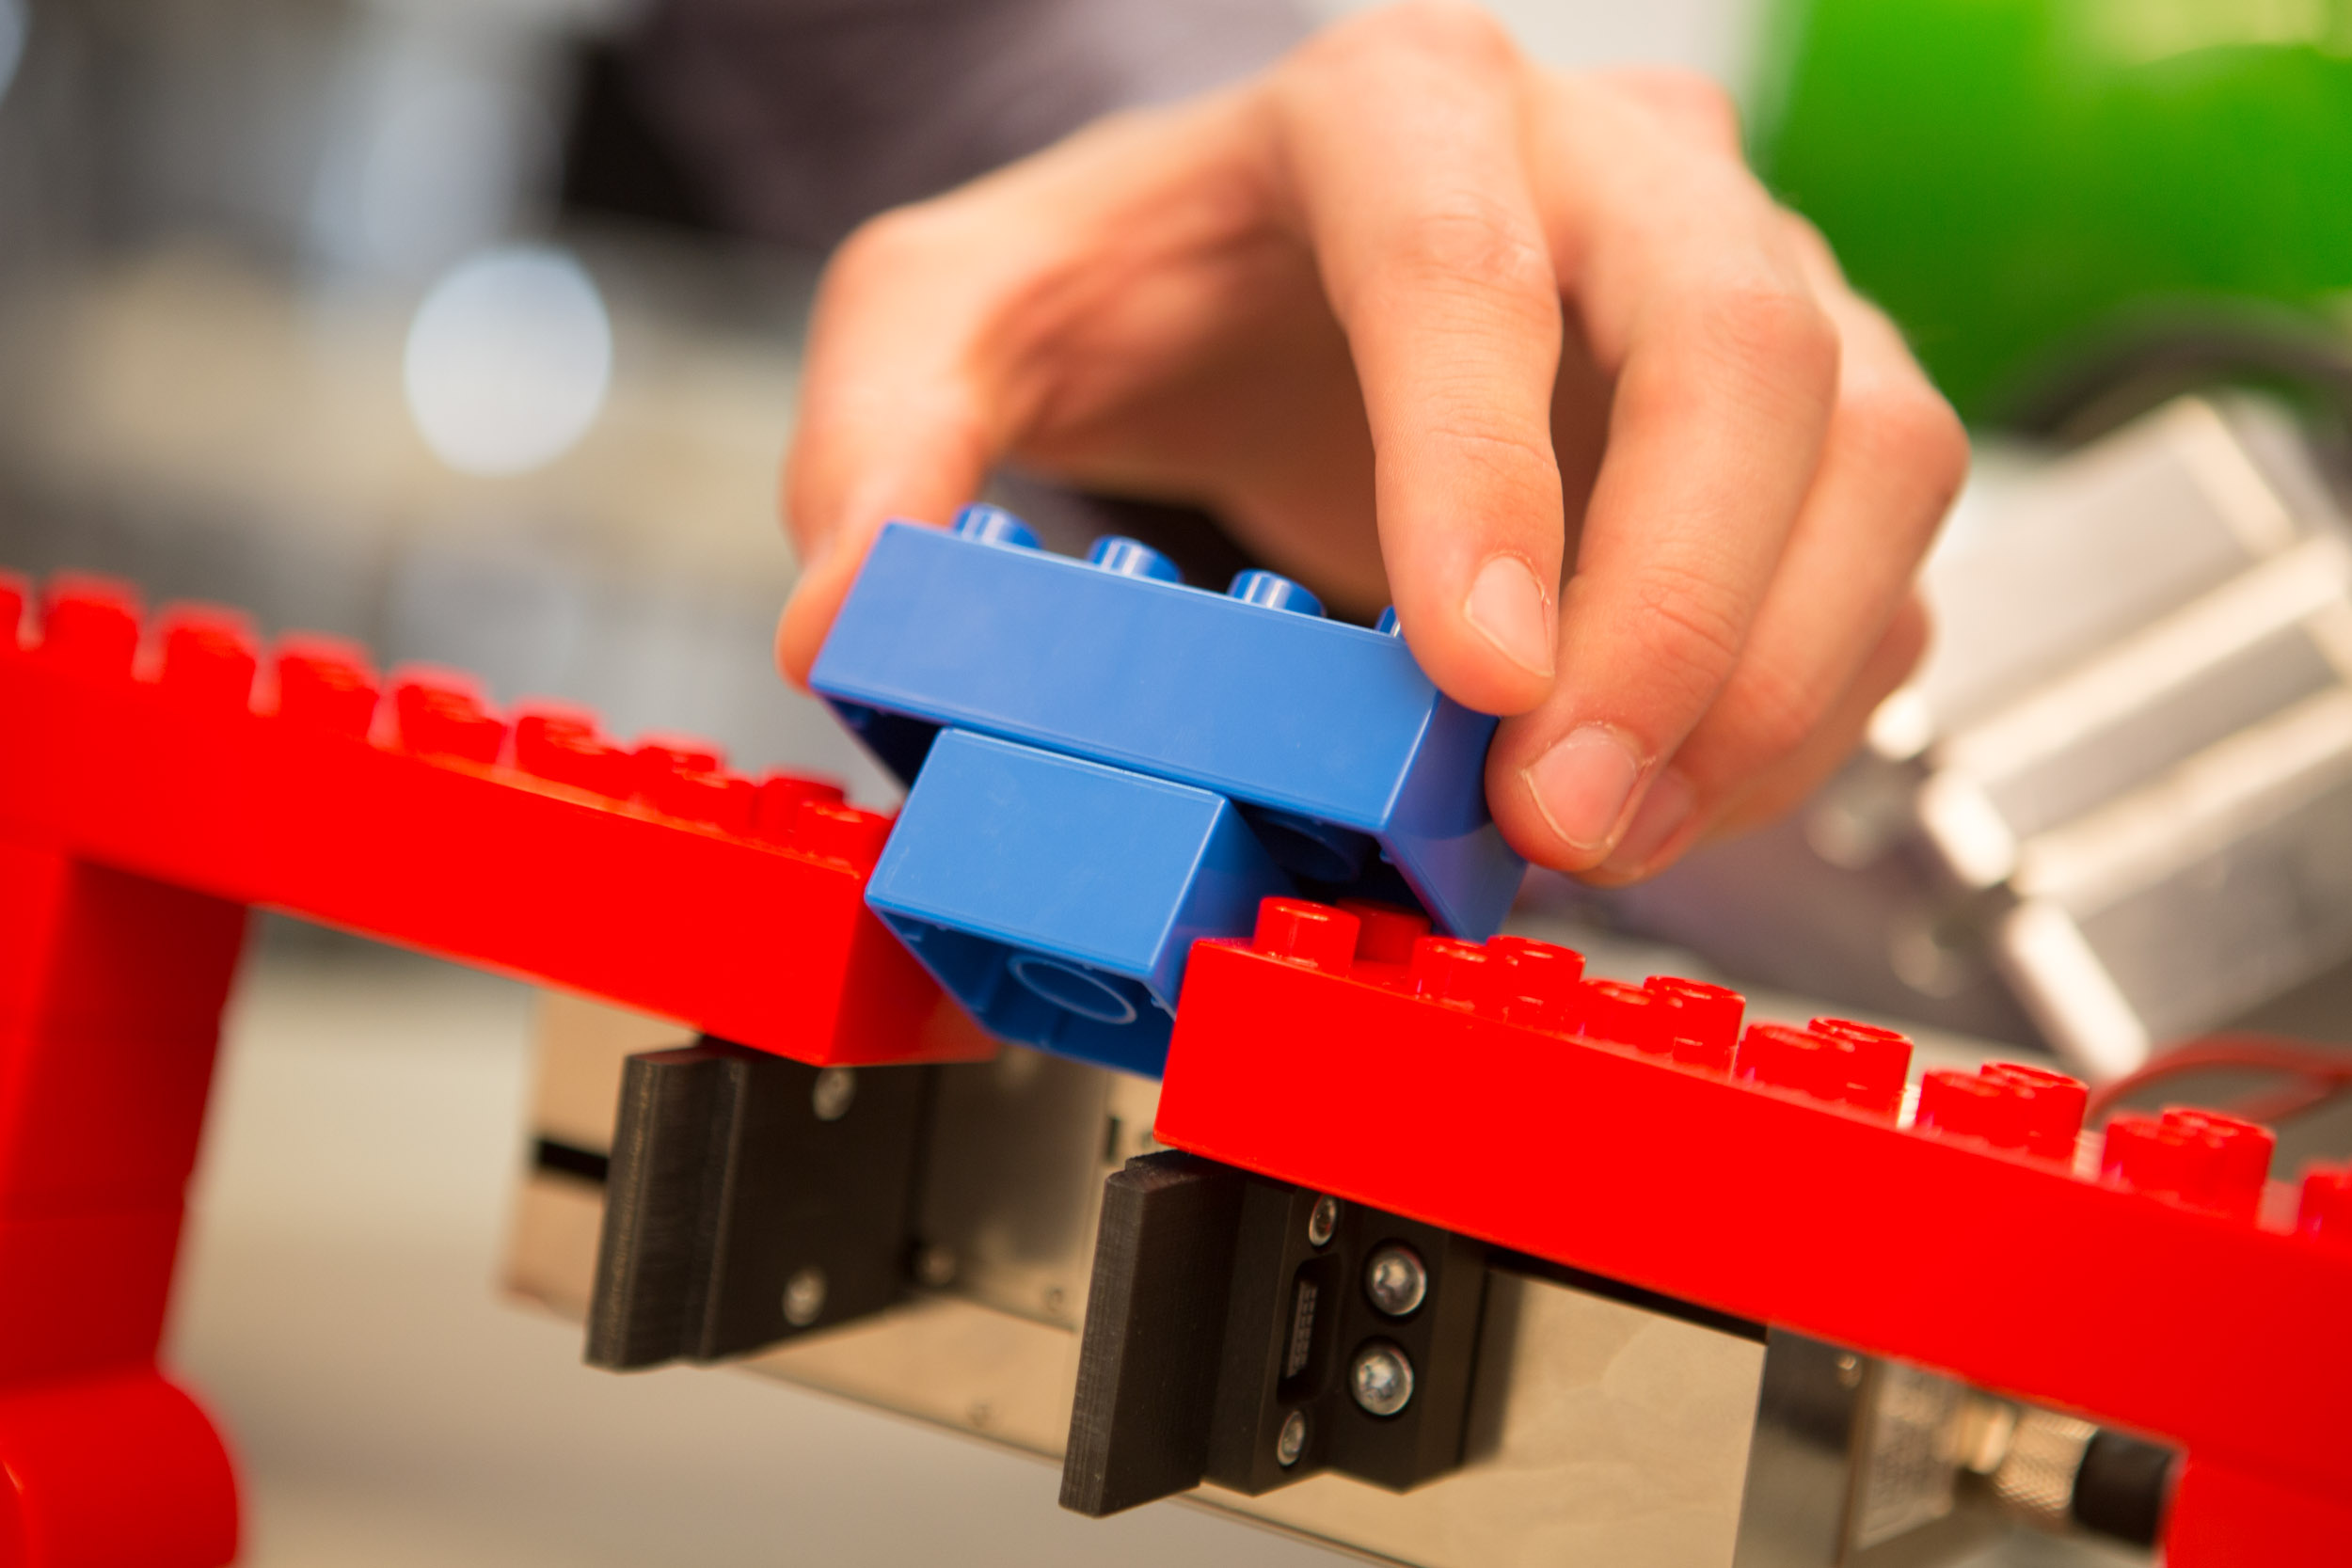
\includegraphics[width=0.3\textwidth] {Lego_robot3}
   \label{fig:subfig1}
 }
\quad % puts next subfigure right next to the previous subfigure
\subfigure[Subfigure 2 caption]{
   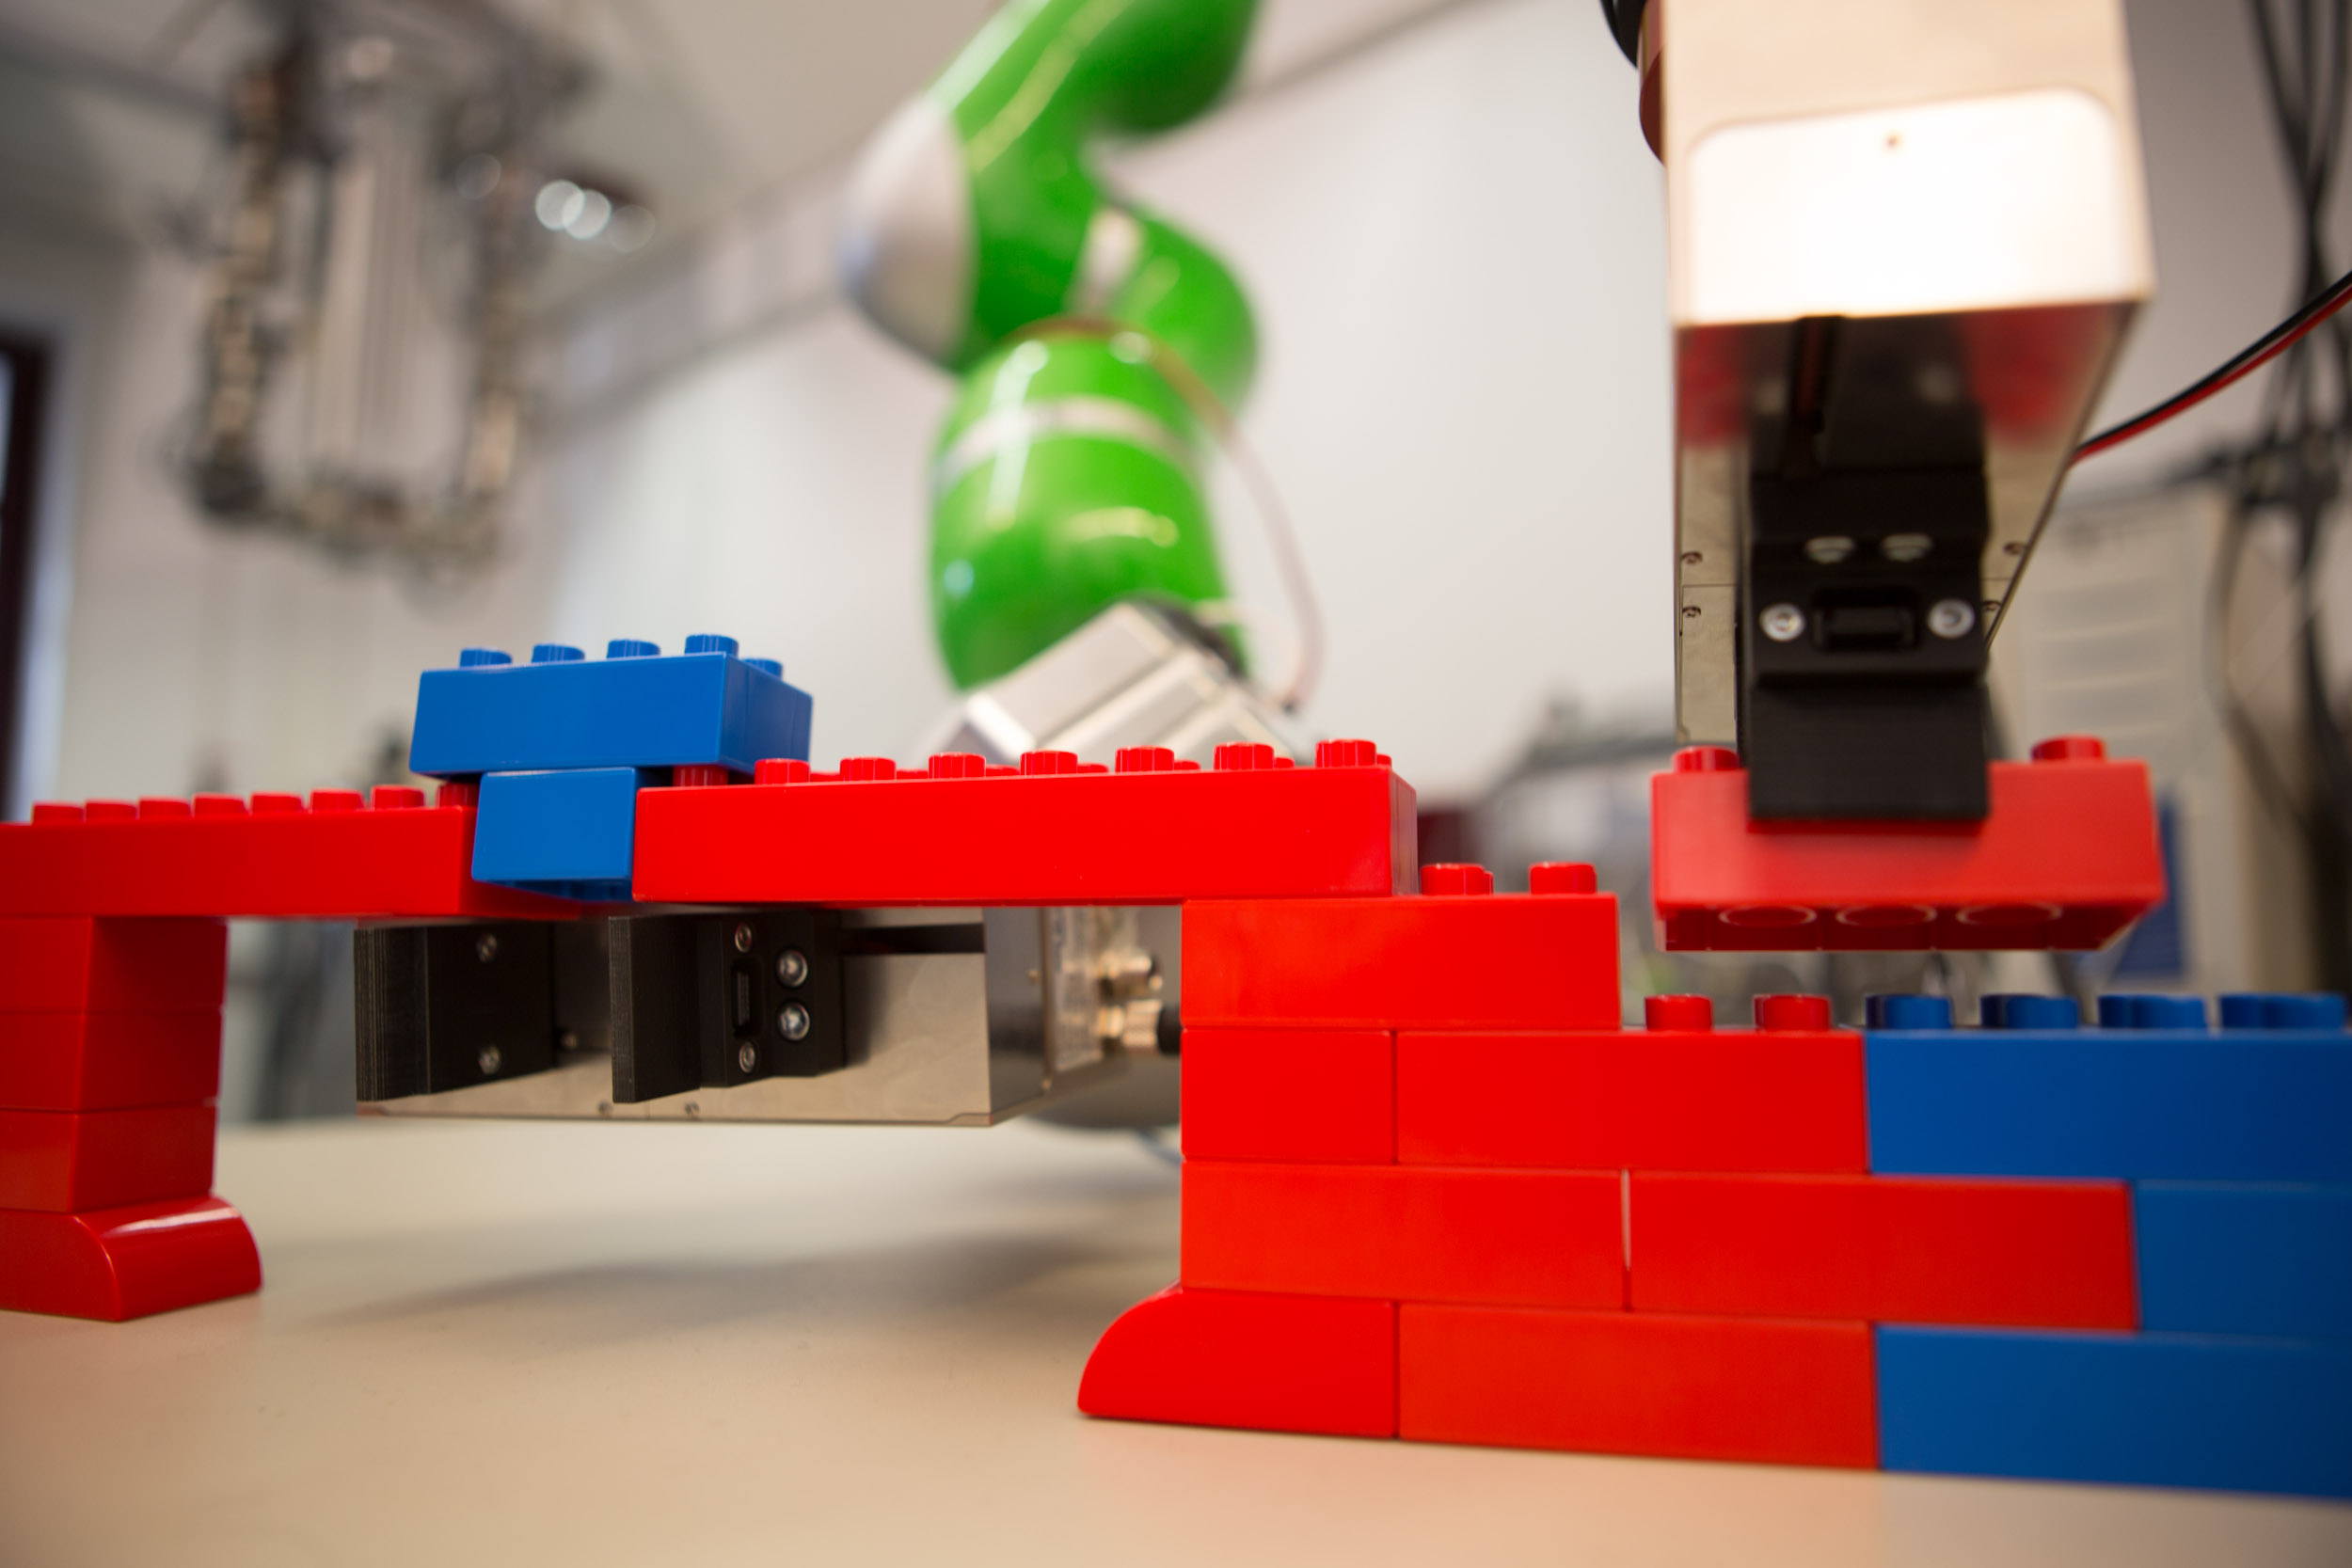
\includegraphics[width=0.3\textwidth] {robot_build}
   \label{fig:subfig2}
 }

\subfigure[Subfigure 3 caption]{
   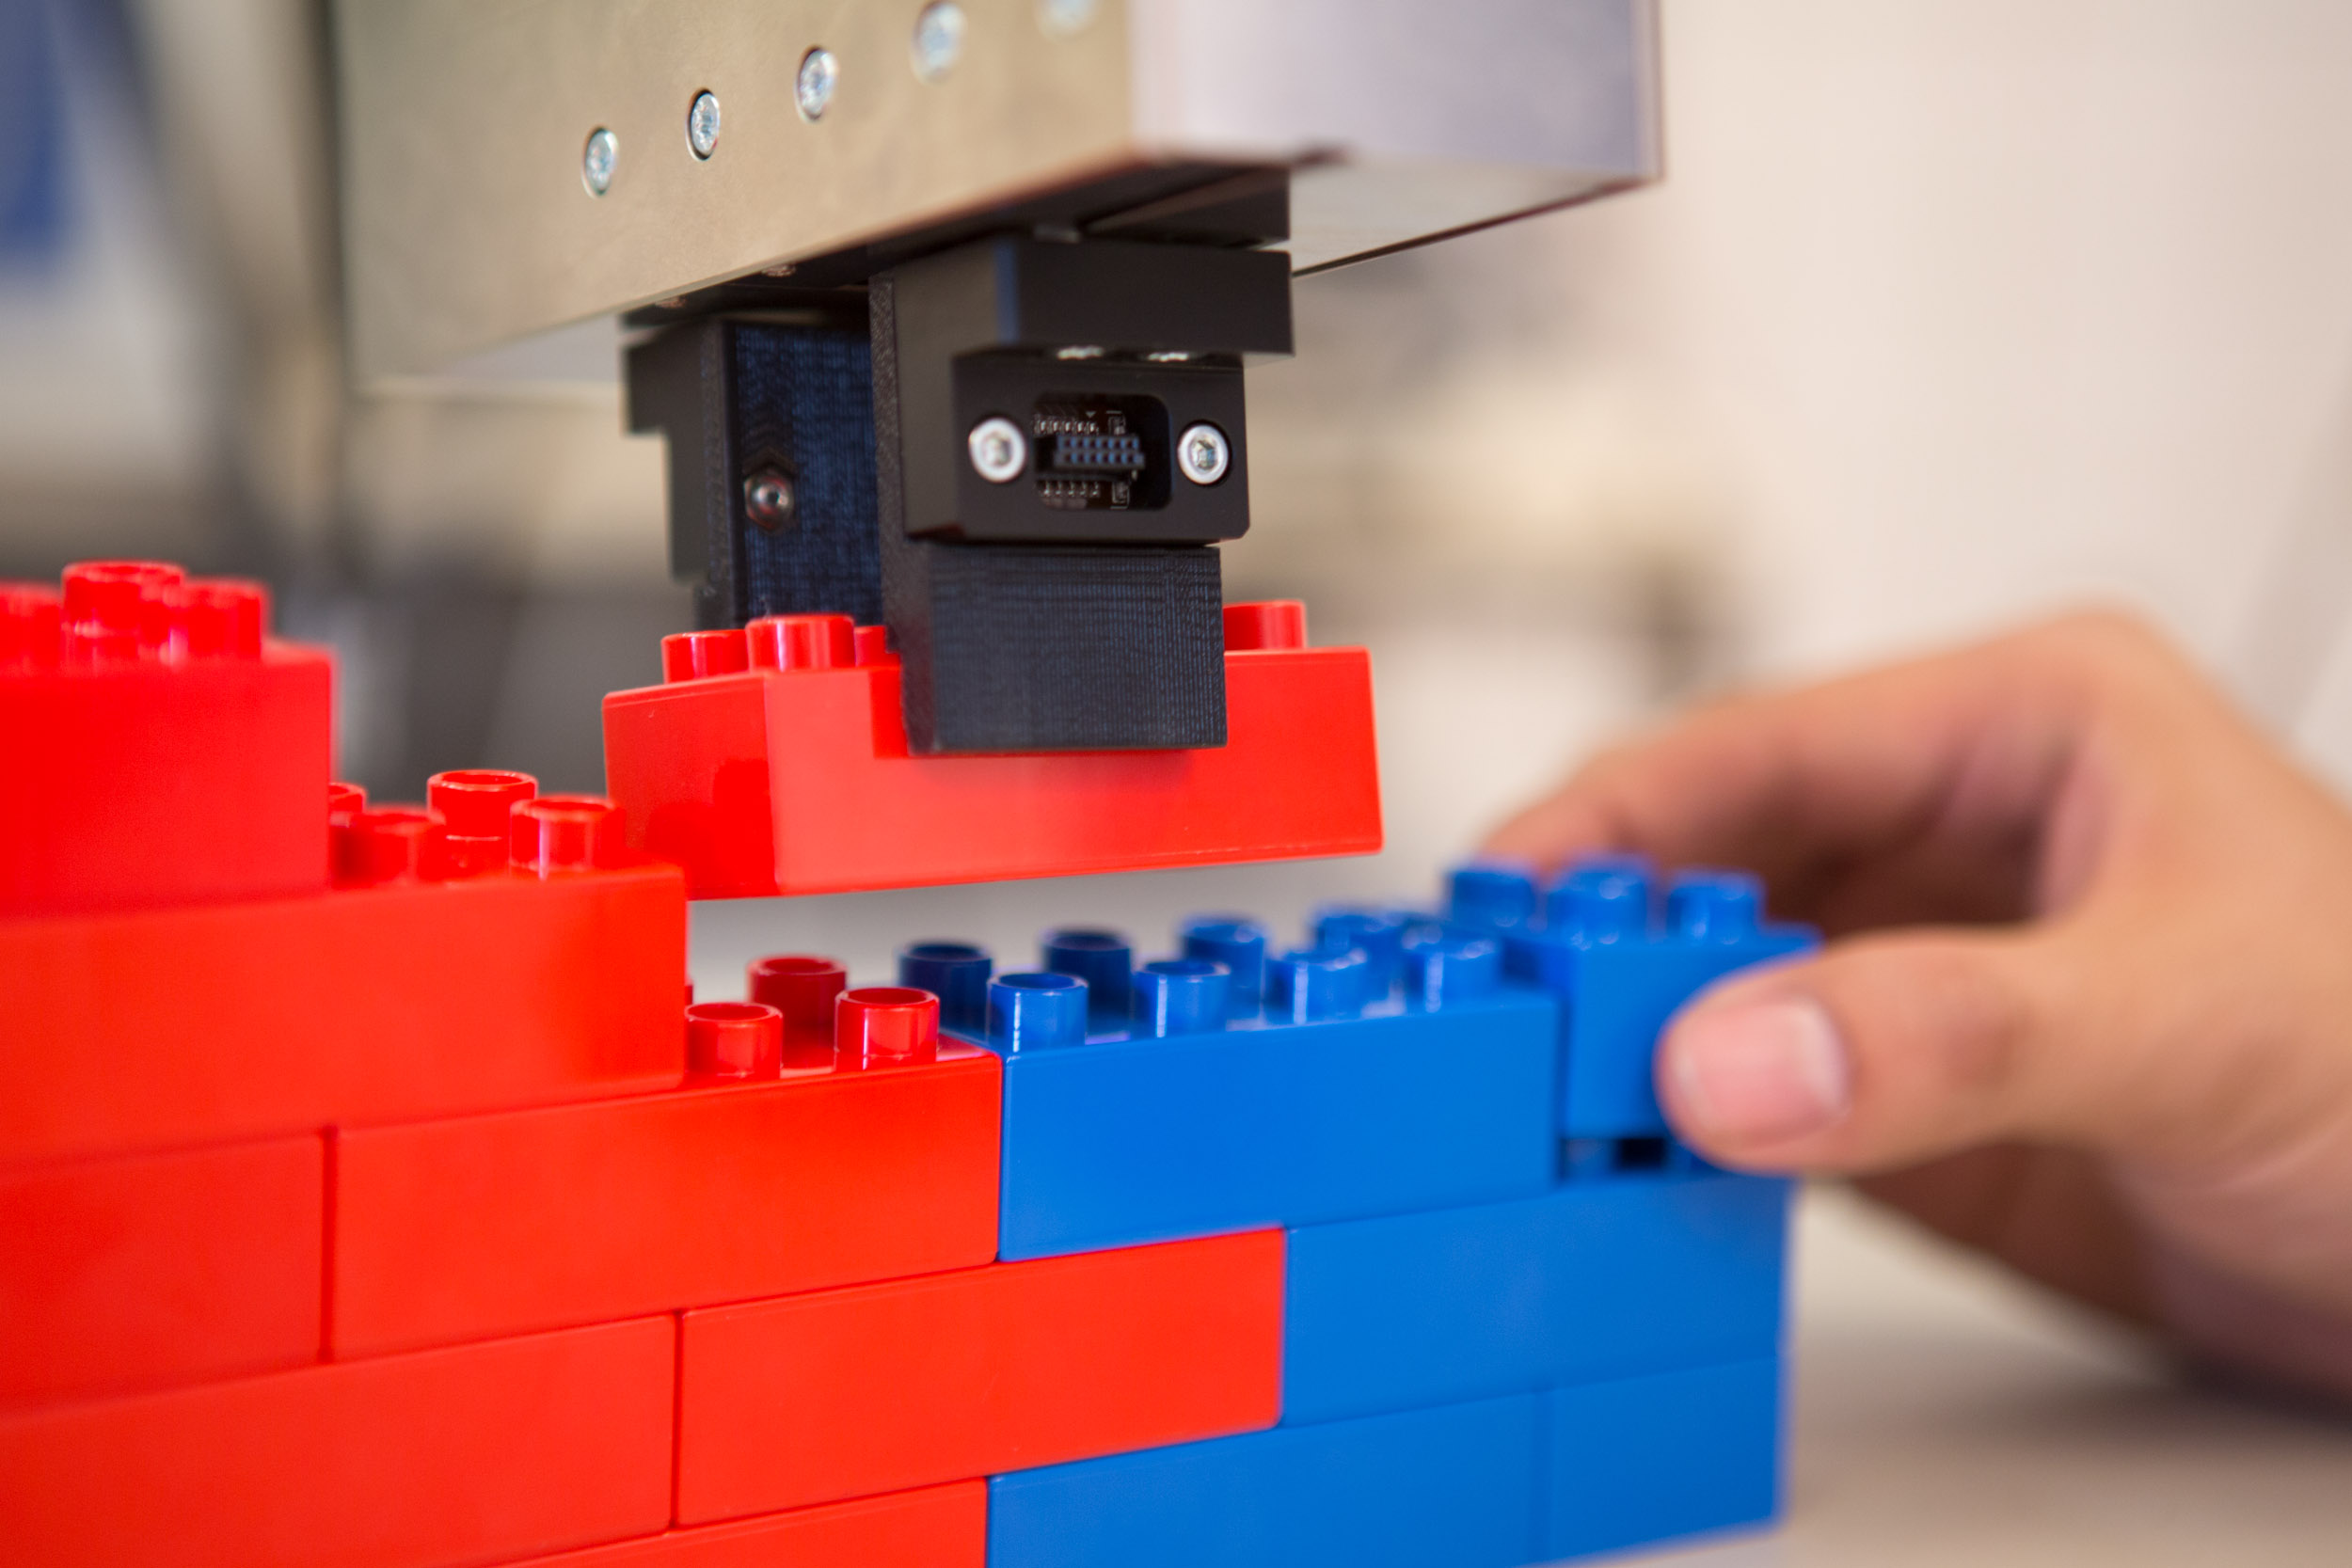
\includegraphics[width=0.4\textwidth] {robot_build_withHuman}
   \label{fig:subfig3}
}
\subfigure[Space-holder for missing picture]{
	\missingfigure[figwidth=0.4\textwidth]{
		\tiny{A Picture needs to be  put here later. One can use acronyms, e.g. \acs{HRC}}}
	\label{fig:subfig4}
}  
\caption[Abbrev. Descr. of subfigure-figure]{A figure with two subfigures}
\label{fig:OverallPic}
\end{figure}

This figures can be referenced by either referencing the overall label \ref{fig:OverallPic} or a specific subfigure label \ref{fig:subfig1} - if the labels have been set properly of course! The subfigures are not listed in the list of figures!

\section{Definitions / Assumptions / Theorems / Lemmas}

Sometimes a definition is helpful, especially for later reference. Motivate and introduce each one and do not just list definitions one after another. Explain why it is important and what it is used for. Assumptions are useful to emphasize what preliminaries have to be fulfilled for your approach to work, especially if you plan to introduce theorems,lemmas,etc . 

Points to remember:
\begin{itemize}
	\item Do not list assumptions one after another. 
	\item Motivate and introduce each one.
	\item Explain how restrictive it is and illustrate its effects on the application.
\end{itemize}

Sometimes you need to cite a theorem/lemma/proposition. 

Points to remember:
\begin{itemize}
	\item Same as above: do not just list, motivate, introduce, explain what this enables.
	\item Make yourself familiar with the way theorems/... are usually formulated. Look at the literature. 
	\item Make sure all relevant assumptions and preliminaries are stated in the theorem/...
	\item Make the proof (if it is your own theorem/...) conclusive and understandable.
\end{itemize}



\section{Citations}

Citations are extremely important and \textbf{must} be included whenever you use other people's work. Direct citations with directly copy-pasting the content and marking it with ``$\ldots$'' are unusual in scientific reports. Always try to reformulate the source into your own words to generate an indirect citation. 


Whether to use numeric or alphabetic references isn't all that important (unless prescribed by a conference or journal), but alphabetic tends to be more readable. Independent of citation style, the following rules should be followed:

\begin{itemize}
\item Use the \LaTeX~cite package. It doesn't give you additional commands, but it fixes a few quirks in \LaTeX. Among others it automatically sorts multiple citations, and it correctly spaces the angular brackets (if you use the \verb|\cite{}| command without leading white space).

\item Citing several papers at one point should be done with a single \verb|\cite{}| command. For example, use \verb|gives good results\cite{Bloe_99, Jay_87}|, resulting in gives good results \cite{Bloe_99, Jay_87}. 

Do not use \verb|gives good results\cite{Bloe_99}\cite{Jay_87}| which produces the ugly gives good results \cite{Bloe_99}\cite{Jay_87}. Also, note that there is no space between the \verb|\cite{}| command and the preceding word, \LaTeX~(with the cite package) does the spacing correctly.

\item Avoid citations of the kind: \cite{Bloe_99} thinks that $x>y$ is valid, but \cite{ONeill_2000} argues that this is invalid in case of $z\geq5$. This works a bit better if using alphanumeric citation labels. Better, though, use the author's names: Bloe and Joe [1] think that $x>y$ is valid, but O'Neill et al. \cite{ONeill_2000} argues that this is invalid in case of $z\geq5$. 

\item Avoid citations at the beginning of a sentence:
	\begin{itemize}
		\item Bad:
		\begin{itemize}
			\item \cite{Bloe_99} introduces different methods for motion control. (citation at the beginning)
			\item Different methods for motion control are introduced in literature. \cite{Bloe_99} (citation after the punctuation)
			\item Different methods for motion control are introduced in\cite{Bloe_99}. (preceding space missing or wrong cite package)
		\end{itemize}
		\item	Good: 	 
		\begin{itemize}
			\item Different methods for motion control are introduced in \cite{Bloe_99}.
			\item Khalil et al. introduce different methods for motion control \cite{Bloe_99}. 
			\item Motion control as in \cite{Bloe_99} is generally used to $\ldots$ .
			\item Motion control \cite{Bloe_99} is generally used to $\ldots$ .
			\item Motion control is generally used to $\ldots$ \cite{Bloe_99}.
		\end{itemize}
	\end{itemize}


\item BibTeX is a great tool, but you need to know how to use it. A regular trap is to forget that \TeX~knows more about typesetting than you do. So, for example, it changes the case of words in the title. If your title contains acronyms and proper names (most do), they tend to get down-cased. Any such words which should not have their case changed should be put into braces, e.g., \verb|{The {Mungi} {OS} and its Use in Merry-Go-Round Seat Allocation}|.


\item In citations don't abuse the category technical report. People tend to cite just about anything that hasn't been published in a journal or conferences as a TR. This is outright wrong. The concept of a TR is actually fairly well defined: A TR is published in some sort. This is generally as part of a formal TR series of some institution, in hardcopy or on the web or both. (They aren't always called ``technical report'', other common names are ``research report'', ``technical memorandum'', $<$institution$>$ ``report'' etc.) The publication (i.e. availability outside) is essential, otherwise it's at best an internal report.
A TR has a number (absolutely!), an institution (publisher), a date (month and year at least) and a publisher's address (besides all the other stuff bibentries have).
If your document doesn't have these features, it's not a TR. It's probably better categorized as a working paper. Even then it has a date and an institution address.

\item Citing web pages is often unavoidable (but also often a sign of laziness). When citing web pages be aware that they may only be short-lived. Consider whether the reference will be of any use to the reader at all if the link is broken. Or whether your whole document only has a use-by date a few months past writing.

\end{itemize}

Any cited document, whatever it may be, has a few \textbf{mandatory} features:
\begin{itemize}
	\item Date. Absolutely. 
	\item Author/organization/creator/person responsible for contents.
	\item Whatever information the reader needs to find that document. In most BibTeX entry types these are clearly identified as mandatory fields. Mandatory means that they aren't optional. Don't pretend they are. For a working paper these might be the contact details of the author.
\end{itemize}


For bibliography, edit {\tt mybib.bib} and list all
references in a special style, e.g. for a book: 
\begin{verbatim}
@book{literaturstelle1,
 author    = {S. Sastry},
 title     = {Nonlinear Systems - Analysis, Stability, and Control},
 publisher = {Springer},
 year      = 1999
}
\end{verbatim}

Cite references in the text by \verb|\cite{citationreference}|.

In order to have your references shown in your PDF, compile by:

\begin{verbatim} 
latex myfile
bibtex myfile
latex myfile
latex  myfile
dvips myfile
ps2pdf -sPAPERSIZE=a4 myfile.ps
\end{verbatim}

Alternatively you can use your preferred \LaTeX -editor. The according BibTeX compiler has to be configured properly and then run before running PdfLaTeX. We recommend you to use our preconfigured editors.

\section{Compiling}
Linux: 
do the following in a Shell:\\
\begin{verbatim}
latex myfile
dvips myfile
ps2pdf -sPAPERSIZE=a4 myfile.ps
\end{verbatim}
Make sure to use the A4 option, when you print the pdf!

Alternatively you can use either Kile, Texmaker, etc. on Linux or TeXnic Centre, etc. on Windows. Please be aware you have to set the required \LaTeX paths in your editors. The most common \LaTeX -editors in Linux are preconfigured at LSR and should work \emph{out-of-the-box}.





\fi
%_________Einleitung__________________________________
\chapter{Introduction}

Your first chapter in the document.
Introduce the problem (gently!). Try to give the reader an appreciation of the difficulty, and an idea of how you will go about it. It's like the overture of an opera: it plays on all the relevant themes.

Make sure you clearly state the vision/aims of your work, what problem you are trying to solve, and why it is important. While the introduction is the part that is read first (ignoring title and abstract) it is usually best written last (when you actually know what you have really achieved). Remember, it's the first thing that is being read, and will have a major influence on the how the reader approaches your work. If you bore them now, you've most likely lost them already. If you make outrageous claims pretend to solve the world's problems, etc, you're likely fighting an uphill battle later on. Also, make sure you pick up any threads spun in the introduction later on, to ensure that the reader thinks they get what they have been promised. Don't create an expectation that you'll deliver more than you actually do. Remember, the reader may be your marker (of a thesis) or referee (of a paper), and you don't want to annoy them.

\section{Problem Statement}

You can either state the problem you are trying to solve in the general introduction, providing the transition from the overall picture to your specific approach, or state it in a separate section. Even if you don't use the separate section, writing down in a few sentences why the problem you are trying to solve is actually hard and hasn't been solved before can give you a better idea of how to approach the topic. This can be also merged with the related work part.

\section{Related Work}

From Kevin Elphinstone's \emph{A Small Guide to Writing Your Thesis}\cite{Elphinstone2014}:

``The related work section (sometimes called literature review) is just that, a review of work related to the problem you are attempting to solve. It should identify and evaluate past approaches to the problem. It should also identify similar solutions to yours that have been applied to other problems not necessarily directly related to the one your solving. Reviewing the successes or limitations of your proposed solution in other contexts provides important understanding that should result in avoiding past mistakes, taking advantage of previous successes, and most importantly, potentially improving your solution or the technique in general when applied in your context and others.

In addition to the obvious purpose indicated, the related work section also can serve to:

\begin{itemize}
	\item justify that the problem exists by example and argument
	\item motivate interest in your work by demonstrating relevance and importance
	\item identify the important issues
	\item provide background to your solution
\end{itemize}

Any remaining doubts over the existence, justification, motivation, or relevance of your thesis topic or problem at the end of the introduction should be gone by the end of related work section.

Note that a literature review is just that, a review. It is not a list of papers and a description of their contents! A literature review should critique, categorize, evaluate, and summarize work related to your thesis. Related work is also not a brain dump of everything you know in the field. You are not writing a textbook; only include information directly related to your topic, problem, or solution.''

Note: Do the literature review at an early stage of your project to build on the knowledge of others, not reinvent the wheel over and over again! There is nothing more frustrating after weeks or months of hard work to find that your great solution has been published 5 years ago and is considered old news or that there is a method known that produces superior results.

%____________________________________________________
\chapter{Technical Approach}

\section{Design of your solution}

Having explained the problem, and what others have done in similar situations, now explain your approach. Again, give a general overview of your design first, and then go into detail. The important part here is the concept of your work, not the actual implementation! Make sure that the document (particularly a thesis) is self-contained: It should be possible for a reader familiar with the general area to understand your design. Again, be forthright about the limitations of your design. Also, make sure you justify any shortcuts/limitations convincingly.

\section{Implementation}

In many (not all cases) there is a clear difference between the general approach (design) and its implementation in your particular circumstances. The design may be more general than what you can do given time and resources. Or you have developed a general design, and are now implementing a prototype on particular hardware. Give all required details. It should be possible to understand all this without referring to the source code. 

This will, in general, include extracts of actual algorithms and hardware components used. Don't list pages of C code, an electronic copy of the source will accompany the submission and should be available to the marker, so there's no point in killing extra trees to put it into the report. Source code, if included at all, goes into the appendix and not the main document.

Make sure you describe your implementation in enough detail. Someone who has nothing else but your thesis report to go by should be able to repeat your work, and arrive at essentially the same implementation. Reproducibility is an important component of scientific work. Also, clearly state the limitations of your implementation, and justify them.



\chapter{Evaluation}

\section{Experimental Results}

A thesis almost always has an experimental part, typically some comparison to other approaches. Benchmarking takes time, for running the experiments, but also for thinking them up in the first place, and for analysing the results. Plan accordingly to spend enough time here!

Think about what makes sense to measure, what you want to learn from your measurements. Think about what is really the relevant contribution of your thesis, and how you can prove that you have achieved your goals. Think about what you can measure in order to get a good insight into the performance of various aspects of your design, how you can distinguish between systematic and accidental effects, how you can convince yourself that your results are right. If you get surprising results, don't just say ``surprise, surprise, performance isn't as good as hoped''. Find out why. Surprises without explanation indicate either that you are clueless about what's going on, or that you have made a mistake. Unconvincing results, therefore, tend to imply unconvincing marks. 

\paragraph{Statistics:} Measurements always have statistical (sampling) errors. Owing to the deterministic nature of simulations these are sometimes very small, as disturbing factors can be designed. However, the reader should be given an indication of how statistically significant the results are. This is done by providing at least a standard deviation in addition to averages. Whenever the results of several runs are averaged, a standard deviation can (and must) be supplied. After all, you average to reduce statistical errors.

The reproducibility argument applies here just as much as for the implementation. Give enough detail on what you measure, and how you measure it, so that someone who has your implementation (but not your test code) or has re-done your implementation independently, should be able to repeat your measurements and arrive at essentially the same results. In some cases, results seem outright wrong in a thesis. In those cases, not enough detail is provided to allow the supervisor/reader to pinpoint the likely source of the error. Often the cause is systematic errors resulting from an incorrect measurement technique. If it seems wrong, and the text doesn't convince the reader that it is not wrong, the reader will assume that it is wrong.


\chapter{Discussion}

Discuss and explain your results. Show how they support your thesis (or, if they don't, give a convincing explanation). It is important to separate objective facts clearly from their discussion (which is bound to contain subjective opinion). If the reader doesn't understand your results, reconsider if you have managed to extract the core information and explain it in a straightforward way.

%_______________________________________________

%_____Zusammenfassung, Ausblick_________________________________
\chapter{Conclusion}

Don't leave it at the discussion: discuss what you/the reader can learn from the results. Draw some real conclusions. Separate discussion/interpretation of the results clearly from the conclusions you draw from them. (So-called ``conclusion creep'' tends to upset reviewers. It means surrendering your scientific objectivity.) Identify all shortcomings/limitations of your work, and discuss how they could be fixed (``future work''). It is not a sign of weakness of your work, if you clearly analyse and state the limitations. Informed readers will notice them anyway and draw their own conclusions, if not addressed properly.

\vspace{\baselineskip}
Recap: don't stick to this structure at all cost. Also, remember that the thesis must be:

\begin{itemize}
	\item honest, stating clearly all limitations;
	\item self--contained, don't write just for the locals, don't assume that the reader has read the same literature as you, don't let the reader work out the details for themselves.
\end{itemize}

This chapter is followed by the list of figures and the bibliography. If you are using acronyms, listing them (with the expanded full name) before the bibliography is also a good idea. The acronyms package helps with consistency and an automatic listing.


\appendix
	%_________Appendix__________________________________
\ifLSRITRtutorial
	\chapter{BUSTED! Last chance to actually read the HowTo-Section!!}
	
	Make sure your thesis is well structured, that each major section does what it is supposed to do, and that the whole thing hangs together. The basic structure is often as given in this template (but other structures are possible). In particular, don't think you need to have exactly as many major sections or chapters as the list implies; sometimes it makes sense to merge things, sometimes it makes sense to move things (e.g., the literature review is in many papers deferred until after the results), sometimes it makes sense to split a logical part into several individual sections. Just use some common sense.
	
	Hand in your thesis at minimum \textbf{one week} before the deadline for correction. You will receive feedback for the final version and very likely have to do minor or major revisions of your writing. Plan your writing schedule to allow for these adjustments, which can have quite some impact on your grade! 
	
	\optional{Please have a look on our \href{https://wiki.lsr.ei.tum.de/thesiswriting_students}{thesis-guidelines} as well before submitting your \emph{final} thesis.}
	
	\section{Style and Expressions}
	
	Before handing in your thesis, even for an intermediate review, please perform a spellcheck and correct grammar mistakes. The report is not meant to be a narrative text. Please stick to neutral and technical style and avoid subjective or biased expressions or adjectives/adverbs such as \emph{obviously, always, very, especially well, actually, so-called etc}. Scientific writing is about precision and you should underpin your statements factually, not soften them with unnecessary qualifiers.
	
	... Okay enough. But please check chapter \ref{sec:Tutorial} before starting with your report. 
\fi
%%%%%%%%%%%%%%%%%%_Abbildungsverzeichnis %%%%%%%%%%%%%%%%%%%%%%
\cleardoublepage
\addcontentsline{toc}{chapter}{List of Figures} 
\listoffigures 	

%%%%%%%%%%%%%%%%%%_List of Tables %%%%%%%%%%%%%%%%%%%%%%
% A lit of tables can be added - if wanted and needed by commenting out the lines below
% \cleardoublepage
% \addcontentsline{toc}{chapter}{List of Tables} 
% \listoftables	

%%%%%%%%%%%%%%%%%%_Acronyms and Notations %%%%%%%%%%%%%%%%%%%%%%
\cleardoublepage
%ifdefined\AddMyGloss
\AddMyGloss 
% --> see include/gloss.tex
%\fi

%%%%%%%%%%%%%%%%%%Literaturverzeichnis %%%%%%%%%%%%%%%%%%%%%%%%
\cleardoublepage
\addcontentsline{toc}{chapter}{Bibliography}
\bibliography{./refs/mybib}
\bibliographystyle{alphaurl}

%%%%%%%%%%%%%%%%%%%%License %%%%%%%%%%%%%%%%%%%%%%%%%%%%%%%%%%%
\cleardoublepage
\chapter*{License}
\markright{LICENSE}
This work is licensed under the Creative Commons Attribution 3.0 Germany
License. To view a copy of this license,
visit \href{http://creativecommons.org/licenses/by/3.0/de/}{http://creativecommons.org} or send a letter
to Creative Commons, 171 Second Street, Suite 300, San
Francisco, California 94105, USA.

%%%%%%%%%%%%%%%%%%%%List of TODOs %%%%%%%%%%%%%%%%%%%%%%%%%%%%%%%%%%%
% this MUST be empty and removed in the final version of course!
\listoftodos
\end{document}
